\begin{figure}[h] % h means place here if possible
\centering
\def\layersep{2.5cm}
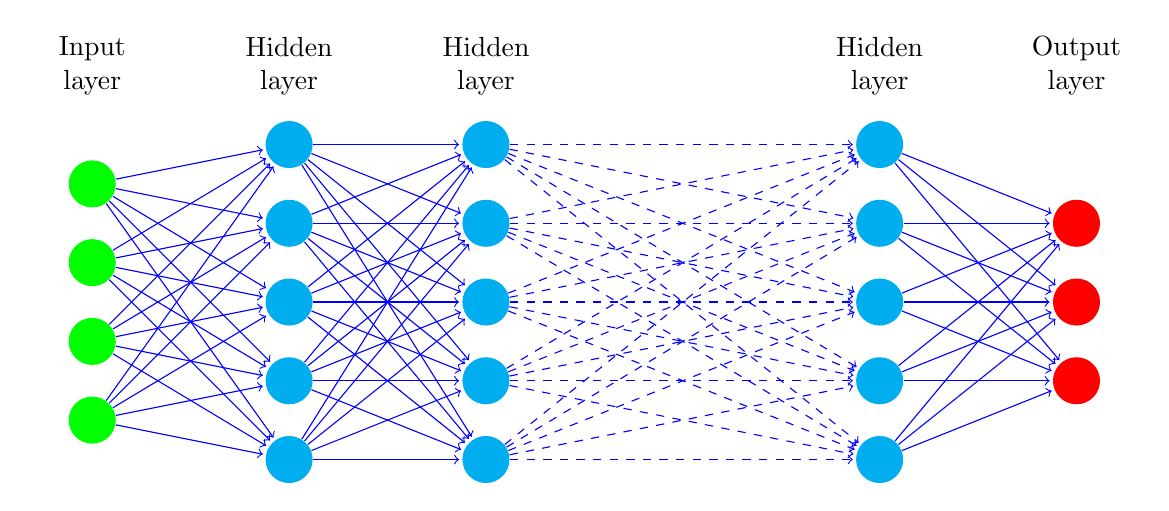
\begin{tikzpicture}[shorten >=1pt,->,draw=blue, node distance=\layersep]
    \tikzstyle{every pin edge}=[<-,shorten <=1pt]
    \tikzstyle{neuron}=[circle,fill=black!25,minimum size=17pt,inner sep=0pt]
    \tikzstyle{input neuron}=[neuron, fill=green];
    \tikzstyle{output neuron}=[neuron, fill=red];
    \tikzstyle{hidden neuron}=[neuron, fill=cyan];
    \tikzstyle{annot} = [text width=4em, text centered];

    % Determining the input layer.
    \node[input neuron] (I-1) at (0,-1) {}; % {$T_{2m}$};
    \node[input neuron] (I-2) at (0,-2) {}; % {$q_v$};
    \node[input neuron] (I-3) at (0,-3) {}; % {$RH$};
    \node[input neuron] (I-4) at (0,-4) {}; % {$p_s$};

    % Draw the input layer nodes
    %\foreach \name / \y in {1,...,4}
    % This is the same as writing \foreach \name / \y in {1/1,2/2,3/3,4/4}
    %    \node[input neuron, pin=left:Input \#\y] (I-\name) at (0,-\y) {};

    % Draw the hidden layer nodes
    \foreach \name / \y in {1,...,5}
        \path[yshift=0.5cm]
            node[hidden neuron] (H-\name) at (\layersep,-\y cm) {};

    % Connect every node in the input layer with every node in the
    % hidden layer.
    \foreach \source in {1,...,4}
        \foreach \dest in {1,...,5}
            \path (I-\source) edge (H-\dest);

    % Draw the hidden layer nodes
    \foreach \name / \y in {1,...,5}
        \path[yshift=0.5cm]
            node[hidden neuron] (R-\name) at (2*\layersep,-\y cm) {};

    % Connect every node in the input layer with every node in the
    % hidden layer.
    \foreach \source in {1,...,5}
        \foreach \dest in {1,...,5}
            \path (H-\source) edge (R-\dest);

    % Draw the hidden layer nodes
    %\foreach \name / \y in {1,...,5}
    %    \path[yshift=0.5cm]
    %        node[hidden neuron] (T-\name) at (3*\layersep,-\y cm) {};

    % Draw the hidden layer nodes
    \foreach \name / \y in {1,...,5}
        \path[yshift=0.5cm]
            node[hidden neuron] (L-\name) at (4*\layersep,-\y cm) {};

    % Connect every node in the input layer with every node in the
    % hidden layer.
    \foreach \source in {1,...,5}
        \foreach \dest in {1,...,5}
            \path[dashed] (R-\source) edge (L-\dest);



    % Connect every node in the input layer with every node in the
    % hidden layer.
    %\foreach \source in {1,...,5}
    %    \foreach \dest in {1,...,5}
    %        \path (R-\source) edge (T-\dest);



    % Draw the output layer node
    \node[output neuron, right of=L-2] (o1) {};
    \node[output neuron, right of=L-3] (o2) {};
    \node[output neuron, right of=L-4] (o3) {};

    % Connect every node in the hidden layer with the output layer
    \foreach \source in {1,...,5}
        \foreach \dest in {1,...,3}
            \path (L-\source) edge (o\dest);

    % Annotate the layers
    \node[annot,above of=H-1, node distance=1cm] (hl) {Hidden layer};
    \node[annot,above of=R-1, node distance=1cm] (hr) {Hidden layer};
    %\node[annot,above of=T-1, node distance=1cm] (ht) {Hidden layer};
    \node[annot,above of=L-1, node distance=1cm] (hL) {Hidden layer};

    \node[annot,left of=hl] {Input layer};
    \node[annot,right of=hL] {Output layer};
\end{tikzpicture}

\caption{Deep fully connected neural network. An extension of the network presented in Figure \ref{fig:one_layer_mlp}. The sketch is based on the example by \citepaper{ffnn}.}
\label{fig:multilayer_mlp}
\end{figure}